\section{Herramienta web}

En este apartado se tratarán los pasos a seguir para desarrollar la herramienta web
 que de visibilidad, acceso y uso al sistema experto.

\subsection{Metodología SCRUM}

Para el desarrollo e implementación de la herramienta web se usó una metodología basada en SCRUM.
 Tendremos un modelo de desarrollo el cual será iterativo e incremental. Dicho modelo tiene
 las siguientes características:

\subsubsection{Iteraciones}

Una iteración también es conocida como "sprint". Estamos hablando de iteraciones dentro del
 proceso de desarrollo cuya duración será de entre 7 y 30 días, dependiendo del número de
 objetivos que se quieran cumplir y la demanda de la planificación. Al finalizar el srpint
 se obtendrá un incremento del producto, lo cual será un resultado válido y con suficiente
 calidad como para poder ser utilizado.

\begin{figure}[htb]
  \centering
    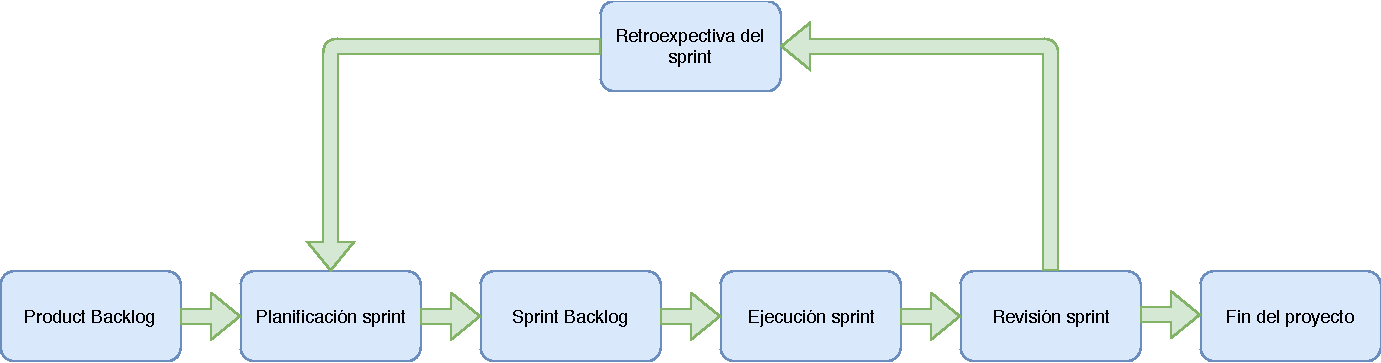
\includegraphics[width=0.4\linewidth]{Scrum}
  \caption[Desarrollo herramienta web]{Desarrollo herramienta web}
  \label{fig:Desarrollo herramienta web}
\end{figure}

Para este proyecto se han utilizado sprints de 30 días para asegurar el cumplimiento de estos.
 La distribución del tiempo fue de 75\% para realizar tareas del sprint en manera de cola de
 prioridad. Dentro de estas tareas se incluye el desarrollo de las pruebas necesarias y la
 comprobación de funcionalidades de las mismas. El resto 25\% se utilizó para el estudio del
 actual sprint para mejora de los siguientes, planificación y organización del siguiente sprint.
 En el capítulo de evaluación encontraremos la tabla con los sprints realizados y la funcionalidad
 desarrollada dentro de este.

\subsubsection{Definición de elementos}

Para la comprensión y buen desarrollo de esta metodología hace falta definir una serie
 de elementos los cuales son los siguientes:

\begin{itemize}
  \item \textbf{Product Backlog:} Será una lista de todos los requisitos del sistema, también
     conocido como historias de usuario. Estos requisitos estarán descritos en alto nivel
     de modo que cualquiera pueda entenderlo y estos estarán priorizados. Esta lista
     podrá verse modificada una vez iniciado el proyecto y en cualquier momento del ciclo de vida.
  \item \textbf{Sprint Backlog:} Esta será la lista de tareas a desarrollar durante el sprint
     para poder llegar al incremento planificado. Cada tarea deberá tener un tiempo estimado
     y los recursos que se necesitan para llevarlas a cabo. Cada tarea no deberá tener una
     estimación mayor de 24 horas puesto que esto indicaría que es demasiado larga y podría
     complicar el cumplimiento del resto de tareas para la fecha acordada. En caso de que
     alguna tarea supere dicho tiempo deberá ser dividida en subtareas.
  \item \textbf{Incremento:} Será el resultado esperado y obtenido al finalizar el sprint. Dicho
     resultado deberá ser terminado y poder ser utilizado.
\end{itemize}

En el caso de este proyecto, el producto backlog estará compuesto desde el principio de todas
 las funcionalidades que se desean implementar. Estas fueron obtenidas a raíz de la metodología
 de desarrollo. Para obtener mayor información sobre dichas funcionalidades deberemos consultar
 el siguiente capítulo en el cual se hablan de las mismas en profundidad.

Estas funcionalidades no serán las únicas en el product backlog puesto que durante el desarrollo
 e implementación del proyecto pueden surgir nuevas que no se hayan identificado en la etapa
 de captura de requisitios. Este caso ocurrio con el desarrollo del manual de usuario,
 informes para mostrar los resultados obtenidos y pequeñas mejoras identificadas al entregar
 el producto al final de cada sprint.

\subsubsection{Definición de roles}

Dentro de un equipo que trabaje en esta metodología habrá dos grupos de personas. El primer grupo
 de personas tendrán los siguientes roles:

\begin{itemize}
  \item \textbf{Product Owner:} Será el encargado de dar voz al cliente. En el caerá la
     responsabilidad de escribir las historias de usuario y ordenarlas en el product backlog.
   \item \textbf{Scrum Master:} Será el encargado de asegurarse que todo va bien en cuanto
      al proceso de desarrollo y este se cumple. Además intentará, en la medida de lo posible,
      evitar el mayor número de incidencias posibles.
   \item \textbf{Equipo:} Serán aquellos que se encarguen de realizar el desarrollo del producto.
\end{itemize}

En este proyecto el tutor del trabajo de fin de grado será quien adopte el rol de product owner
 y scrum master, mientras que el alumno ha sido formado por el autor del proyecto.

El otro grupo no entrará direcamente como parte del proceso, pero habrá que tenerlos en
 cuenta ya que serán ellos quienes nos den información al finalizar el sprint. De esta
 información podremos mejorar nuestro producto, aunque esto conllevará cambios en los
 siguientes sprints. Los usuarios que están dentro de este grupo serán aquellos que usen
 la herramienta, el usuario final. En nuestro caso serán los entrenadores y esgrimistas
 durante las competiciones o entrenamientos.

\subsubsection{Definición de reuniones}

Dentro de scrum existen diferentes tipos de reuniones. Estas reuniones son utilizadas para
 planificar las tareas del sprint, analizar las nuevas tareas que se han de incorporar en
 el product backlog, seguir el estado de salud del sprint y también comprobar cuales fueron
 los resultados de los sprints. Las diferentes reuniones que se llevan a cabo son las siguientes:

\begin{itemize}
  \item \textbf{Planificación del sprint:} En esta reunión se eligen las tareas del product
     backlog según estén ordenadas para mantener la prioridad de estas. Estas tareas deberán
     estar estimadas y hacerlo en caso de que no lo estén. En función del tiempo y recursos
     disponibles para el sprint se deberán escoger mas o menos tareas. Una vez seleccionadas
     tendremos el sprint backlog.
  \item \textbf{Seguimiento del sprint:} Esta será una reunión diaria de muy corta duración.
     El principal objetivo de esta reunión será conocer el estado de salud del sprint, de modo
     que se puedan tomar las medidas oportunas para que todo el trabajo salga adelante. Un
     claro ejemplo sería un bloqueo entre recursos que no se ha detectado previamente. Para
     ello cada miembro del equipo deberá comentar por encima cual fue su trabajo del día
     anterior junto con lo que tiene previsto para la jornada actual. No se deberán abordar
     problemas en esta reunión si se hará fuera de esta. Esta reunión es solo para estar al
     tanto de los posibles problemas.
  \item \textbf{Revisión del sprint:} En esta reunión se revisará el trabajo realizado y cuál
     faltó por completar. Además se presentará el incremento obtenido y se analizará el motivo
     de aquellas tareas que no se terminaron.
\end{itemize}
